\section{Zusatzfragen}
\begin{enumerate}
	\item  \textbf{Warum heißt die hier vorliegende Reaktion Inversionsreaktion ?}\\
	Eine Inversion beschreibt eine chemische Reaktion, die eine Umkehr von bestimmten Eigenschaften der Edukte gegenüber den Produkten bedeutet. 
	In der hier vorliegenden Reaktion ändert sich der Drehwinkel. 
	Saccharose dreht die Ebene des polarisierten Lichtes nach rechts (positiv) und der Invertzucker, bestehend aus Fructose und Glucose, nach links (negativ). 
	Im Verlauf der Reaktion sinkt die Konzentration von Saccharose und die Konzentration vom Invertzucker nimmt zu.\\
	\item \textbf{Wie ist die optische Aktivität mit der Struktur eines Moleküls in Zusammenhang zu bringen ?}\\
	Die meisten Stoffe sind optisch nicht aktiv.
	Da für optische Aktivität ein Chirales Zentrum nötig ist.
	Dies ist der Fall, wenn ein Kohlenstoffatom vier unterschiedliche Liganden hat.
	Chirale Moleküle können nicht mit dem Spiegelbild in Deckung gebracht werden.
	\item \textbf{Welche Bedeutung hat das Messen von Drehwinkeln für die Aufklärung von Reaktionsmechanismen ?}\\
	Wird eine Änderung des Drehwinkels gemessen, so hat eine änderung der Summe an Drehwinkeln, der Reaktionslösung stattgefunden.
	In unserem Fall, da wir Edukt und Produkt kennen, kann so auf den Reaktionsfortschritt geschlossen werden.
	\item \textbf{Wie funktioniert ein Polarimeter ?}\\
	Im Polarimeter misst man den Drehwinkel einer Probensubstanz. 
	Das Licht der Lichtquelle ist linear polarisiert. 
	Wenn die Probe optisch aktiv (chiral) ist, wird das Licht gebeugt. 
	Der drehbare Polarisator stellt die Polarisationsebene fest. 
	Wenn der Drehwinkel des zweiten Polarisationsfilters gleich dem Drehwinkel der Probe entspricht, fällt Licht durch das Polarimeter.
	Siehe Abbildung \ref{abb:polarimeter}.\\
	\item \textbf{Wie wirken sich systematische Fehler bei der Drehwinkelbestimmung auf die erhaltene Werte für $K$ und $E_A$ aus ?}\\
	Es hat keine Auswirkung, da sich die Fehler gegenseitig aufheben. 
\cite{polarimeter}
\end{enumerate}
\newpage

\begin{figure}
\centering
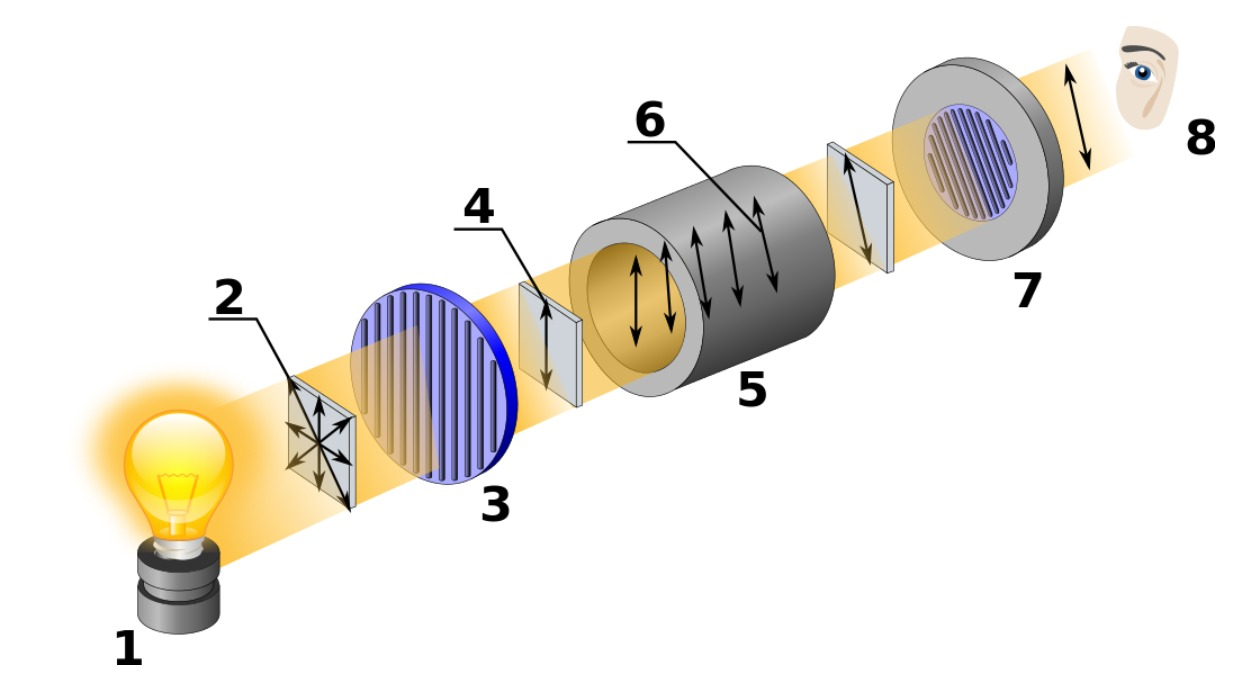
\includegraphics[width=\textwidth]{polarimeter.png}
\caption{Schematische Darstellung des Aufbaus eines Polarimeters}
\label{abb:polarimeter}
\end{figure}
